\documentclass[12pt,a4paper]{article}

\usepackage[utf8]{inputenc}
\usepackage[usenames,dvipsnames,table]{xcolor}
\usepackage{pgfplots}
\usepackage{amsfonts}
\usepackage{rotating}
\usepackage{pdfpages}
\frenchspacing
\usepackage{parskip}
\usepackage{graphicx}
\usepackage[sorting=none,citestyle=ieee,backend=biber]{biblatex}
\usepackage{pgfgantt}
\usepackage{float}
\usepackage{enumitem}
\usepackage[toc,page]{appendix}
\bibliography{progress-report}
\pgfplotsset{compat=1.11}

\title{Investigation Into the Use of Hardware Accelerators in Data Intensive Compute}
\author{CS310 Progress Report\\David Richardson, 1314918}
\date{November 2015}

\begin{document}
	\maketitle
	
	This document details the progress made in the investigation into the use of hardware accelerators in data intensive compute. Section \ref{sec:introduction} reintroduces the project and its aims as well as gives a summary of the project's objectives. Section \ref{sec:research_direction} identifies any existing research in this project's problem domain. Section \ref{sec:benchmarking_progress} details the process for benchmark selection, as well as discusses any progress toward their successful execution. Section \ref{sec:project_management} reiterates the approach to project management as specified in the project specification, giving any necessary changes that have been brought to light by the work so far. Section \ref{sec:further_work_project_extensions} outlines any further work necessary for the project completion and any possible extensions to the project. Finally, Section \ref{sec:conclusion} concludes this progress report by discussing the overall state of this project, as well as reiterating the key points that are to be completed to further its progression. The original specification documentation for this project is available in Appendix \ref{app:specification}.

	\section{Introduction}
	\label{sec:introduction}

        Hardware accelerators are specifically designed computer hardware that are designed to perform some forms of computation, such as floating point arithmetic, faster~\cite{accelerating-matrix-product, quantitative-finance-gpu} and more efficiently~\cite{energy-efficient-gpu} than a general purpose CPU. These accelerators generally take the forms of General Purpose GPUs (GPGPUs) or Many Integrated Core (MIC) co-processors. It is becoming increasingly common to find hardware accelerators installed within the compute nodes of new compute clusters, and with this the possibility for their use is becoming more apparent. Despite this, the amount of research into their use within the paradigm of data intensive compute is underwhelming. The integration of these hardware accelerators into data intensive compute programs, such as MapReduce jobs, could provide benefits such as a decrease in the total compute time and a reduction in the power consumed over the time a program is executing. Other possible benefits involve a reduced need to scale outwards to cope with the Tera- or Petabyte scale data sets that have come about from the data avalanche in areas such as bioinformatics~\cite{big-data-biocuration}. These benefits are of interest to both academic and commercial applications, where it can reduce operational costs and reduce turn around time for compute workloads. Organisations that provide data-centric services such as Google or Facebook would also be able to enrich user experience with features that were previously not feasible due to slow compute times, increasing both value of service and profit.
	
	    \subsection{Project Aims}
	    \label{sub:project_aims}
	    
	        The overarching aim for this project is to investigate and test the use of GPGPU and MIC co-processor accelerators in data intensive workloads, determining if their integration has significant improvements in compute and power consumption versus a CPU-only implementation. Their use has value for both academia and industry, where a reduction in compute time will generally lead to a reduction in operational costs incurred to run a data intensive program. It will also benefit infrastructure management companies such as Amazon, by increasing the performance per Watt of their compute nodes.
	        
	    \subsection{Summary of Objectives}
	    \label{sub:summary_of_objectives}
	    
	        The project has two main objectives that were outlined in the project specification documentation:
	        
	        \begin{enumerate}
	           \item To understand if current benchmarking suites are suitable for hardware accelerated data analytics clusters.
	           \item To determine if accelerators can be used within data analytics with little modification to current software stacks or algorithm implementations.
	        \end{enumerate}
	        
	        Where the notion of a `suitable' benchmark is a benchmark that tests a variety of work loads, makes use of as much of the hardware present in the system as possible like hardware accelerators; and can be scaled in input data set size.
	    
    \section{Research Direction}
    \label{sec:research_direction}
    

        With the project introduced, and its main aims and objectives discussed, the area of related research is now considered.
    
        Research into the use of GPGPU and MIC co-processors within data intensive compute is limited at best, with very few technical reports or articles available.
        
        \subsection{Accelerating Breadth-First Search with Intel MIC Co-processors}
        \label{sub:accelerating_bfs_with_mic}
        
            Tao, Yutong, and Guang provide research into the application of the Intel MIC co-processor architecture to a Breadth-First Search (BFS) of a graph, a common workload in the realm of data intensive compute. Their research considers both native and offload optimisation techniques, giving the optimisation methodologies for both~\cite{mic-accelerate-bfs}. The native optimisation involves performing the BFS entirely on the co-processor and the optimisation techniques used involves the exploitation of thread- and data-level parallelism. The offload optimisation involves the partitioning of the tasks within the workload as well an optimisation of the data communications between CPU and co-processor. They found that their native optimisation could run up to 3.4x faster on two Intel Xeon Phi Knight's Corner than when run on two Intel Xeon E5-2670. Their offload optimisation results in a speed up of up to 1.67x, in comparison. The algorithm used for data communications optimisations in the offload optimisation also benefits greater from larger graph sizes.
    
    \section{Benchmarking Progress}
    \label{sec:benchmarking_progress}
    
        With the nature of this project being mostly based around investigation and research, it is quite hard to measure its progress. However, it is possible to measure progress with regards to the timetable outlined in the project specification, where it lists the key phases to the project. With this in mind, the progress of this project is now discussed.
    
        \subsection{Benchmark Selection}
        \label{sub:benchmark_selection}
        
            There are a number of benchmarking suites available to test, benchmark, and classify data intensive compute clusters. With the paradigm of data intensive compute lacking a `standard' benchmarking suite like LINPACK is to high performance computing, many of these benchmarks also compete to become such a standard. For this project I will be selecting one benchmarking suite for use to compare the effect of the integration of hardware accelerators into them.
            
            Through my investigation into these benchmarks, a few observations have been made:
            
            \begin{enumerate}
                \item Most benchmarking suites come with their own scalable data generators.
                \item All benchmarking suites that have been considered are developed for MapReduce or similar compute workloads.
                \item All benchmarking suites investigated have not been built with the consideration for the use hardware accelerators.
            \end{enumerate}
            
            These observations can be used to conclude about objective 1 that was outlined in the project specification. This is that the current suite of benchmarks are not suitable for hardware accelerated data intensive compute clusters. This is due to the lack of consideration within the benchmarking suites, when developed, for the use of hardware accelerators like GPGPUs and MIC co-processors.
            
            With this in mind, the benchmarking suites that were considered are now discussed and compared.
    
            \subsubsection{Graph500}
            \label{ssub:graph500}
            
                The Graph500 is an initiative to establish a set of large-scale benchmarks for data intensive applications, being backed by both academia and industry experts~\cite{graph500-intro}. At present, the Graph500 benchmark has only one workload that can be separated into two kernels: generating a graph from an edge list, and a breadth-first search of the generated graph~\cite{graph500-spec}. Of these, the second kernel is used as a performance measure of the host system. The second kernel's performance is measured in Traversed Edges per Second (TEPS), providing a standard unit for comparison akin to LINPACK with Floating Point Operations per Second (FLOPS). The reference implementation provided by the Graph500 is written in C and can come in sequential, multi-threaded and multi-process flavours that use standards like OpenMP, XMT and MPI~\cite{graph500-reference-impl}.
        
            \subsubsection{BigDataBench}
            \label{ssub:bigdatabench}

            	BigDataBench is a data analytics benchmarking suite created at the ICT, Chinese Academy of Sciences, with backing from industry partners such as Huawei. The benchmarks in this suite abandon sequential and multi-threaded workloads, that would typically use OpenMP or similar libraries, for scale-out~\cite{big-data-bench-home} workloads that are designed to better represent the distributed nature of data intensive compute. The benchmarks themselves in this suite are derived from a common subset of `dwarf' workloads, such as social network graph analysis or word multimedia analytics~\cite{dwarf-workloads-big-data}. These benchmarks are implemented with MapReduce in mind, using associated frameworks such as Apache Hadoop or Spark. Other implementations are also available that use MySQL and MPI for inter-node communications~\cite{big-data-bench-home}.
            
            \subsubsection{Intel HiBench}
            \label{ssub:intel_hibench}

                Intel's HiBench is a suite of 10 Hadoop-based MapReduce benchmarks that are separated into two categories: synthetic micro-benchmarks and real-world applications~\cite{hibench-techreport}. The suite also takes into account the following 5 system characteristics when benchmarking and classifying a system:

                \begin{itemize}
                    \item Job running time.
                    \item Number of tasks per minute or job throughput.
                    \item HDFS bandwidth.
                    \item Utilisation of system resources like CPU, Memory and I/O.
                    \item Data access patterns
                \end{itemize}

                The suite itself only provides implementations to use Apache's Hadoop framework. The real-world workloads cover web search, machine learning and analytical querying on large data sets. The micro-benchmarks cover basic jobs such as data sorting or extraction of information about a large data set. The suite also includes a benchmark to help determine the aggregated bandwidth that is delivered by HDFS~\cite{hibench-techreport-2}.
            
            \subsubsection{Comparison}
            \label{ssub:comparison}

                With all the benchmarks considered for this project outlined above, they are now compared and a suite will be selected.

                Whilst the Graph500 benchmark is backed by both industry leaders and academics alike, its suite contains only one benchmark that is not wholly representative of data intensive workloads. Its implementation using C and MPI would make the use of hardware accelerators easier on more traditional compute oriented clusters. However, due to Chiron's architecture and chosen software stack, the use of MPI and/or OpenMP would not suit MapReduce and thus the suite will not be used for this project.

                BigDataBench and Intel HiBench both provide extensive suites of benchmarks that can be separated into micro-benchmarks and workloads that are representative of what you would find in use in the real world. BigDataBench has the overall larger number of benchmarks available when compared to HiBench, and the benchmarking suite will also test more than just Apache Hadoop. It doesn't, however, provide the in-depth characterisation of the system that HiBench provides. BigDataBench also has a larger amount of required software, which may make it infeasible to run some benchmarks on Chiron. With these considerations, Intel HiBench will be used for this project based upon its MapReduce workloads and in-depth benchmark reporting.
            
        \subsection{Benchmark Running}
        \label{sub:benchmark_running}

            With the selection of the benchmark suite now complete, it is being used used to provide a baseline performance metric for comparison against the hardware accelerated implementations to come. There have been a few issues found with the lack of software libraries and with the configuration of Chiron when starting the benchmarking procedure. These issues were reported to the Centre of Scientific Computing and were resolved, with little effect to the timetabling of the project due to the provisioning of overrun buffers in the task durations. Only a small subset of benchmarks will be selected from the suite for execution and then adaptation to use hardware accelerators. This is to make it feasible to complete the project within the time given in the timetable.

            Whilst benchmarking, it has also become apparent that the configuration of HDFS on Chiron will make a possible significant impact on the benchmark results. This is because the HDFS volume is partitioned into an SSD partition and a HDD partition, with each differing in total storage size as well as read/write speeds. Due to the nature of data intensive compute being bounded by the speed of I/O, it is not beyond reason that the choice of storage medium would have an effect on results. This can be shown by difference in data access speeds for HDDs using SATA III and SSDs using the M.2 standard with 4x PCI-E 3.0 lanes: 31.56Gbps for M.2~\cite{understanding-pcie} and 6.0Gbps for SATA III~\cite{sata-3-standard}. This results in SATA III being 5.26x slower than M.2 and its 4 PCI-E 3.0 lanes. On top of this, the node interconnects in Chiron are Mellanox InfiniBand with a maximum throughput of 56Gbps~\cite{mellanox-infiniband-manual}, showing that the network will not bottle neck I/O operations and the bottle neck in fact resides with the chosen storage media.
    
    \section{Project Management}
    \label{sec:project_management}

        Having discussed the progress made in the project, attention is now turned to the project's management. The original project management techniques will be reflected upon and any changes to the project timetable or risk assessment will be considered.
    
        \subsection{Timetable}
        \label{sub:timetable}

            In the original project timetable, it was assumed that Chiron would be near or in a production state. With Chiron remaining in a pre-production state, however, it is not without configuration errors and has a lack of user documentation. These issues will, as a result, add possible delays to the project as it moves forwards and the use of untested system components starts to occur. Fortunately the project timetable as given in the specification documentation has some contingencies built into it, in the form of task padding zones marked in red, as well as extra amount of time that allows the project to overrun without issue. Figure~\ref{fig:project-timetable} shows where the project is currently, with any complete tasks in violet. The overrun allowances for benchmark testing and accelerated benchmark testing and analysis have been extended, as well.

            \begin{sidewaysfigure}
                    \centering
                    \begin{ganttchart}[
                        x unit=6mm,
                        hgrid,
                        vgrid,
                        newline shortcut=true,
                        time slot format=simple,
                        bar/.append style={fill=green!15},
                        bar label node/.append style={align=left},
                        milestone inline label node/.append style={right=2mm},
                        milestone/.append style={fill=red},
                        today=9,
                        today offset=0.075,
                        today label=Current Week,
                        today label node/.append style={anchor=north west},
                        today label font=\itshape\color{red},
                        today rule/.style={draw=blue, ultra thick}
                    ]{1}{30}
                        \gantttitle{2015}{12}
                        \gantttitle{2016}{18} \\
                        \gantttitle{Time (in weeks)}{30} \\
                        \gantttitlelist{1,...,30}{1} \\
                        \ganttbar[bar/.append style={fill=violet!25}]{Benchmark selection}{1}{4} \ganttnewline
                        \ganttlinkedbar{Benchmark testing \ganttalignnewline
                            and analysis}{5}{8}
                        \ganttbar[bar/.append style={fill=red!25}]{}{9}{10} \ganttnewline
                        \ganttlinkedbar{Benchmark migration}{11}{14}
                        \ganttbar[bar/.append style={fill=red!25}]{}{15}{15} \ganttnewline
                        \ganttlinkedbar{Accelerated benchmark \ganttalignnewline
                            testing and analysis}{16}{17}
                        \ganttbar[bar/.append style={fill=red!25}]{}{18}{19}
                        \ganttlinkedmilestone[inline=true, milestone/.append style={fill=green}]{Research complete}{20} \ganttnewline[thick, black]
                        \ganttbar[bar/.append style={fill=violet!25}]{Project specification}{1}{2} 
                        \ganttmilestone[inline=true, milestone/.append style={fill=magenta}]{Submission}{2} \ganttnewline
                        \ganttbar[bar/.append style={fill=violet!25}]{Progress report}{6}{8}
                        \ganttmilestone[inline=true, milestone/.append style={fill=magenta}]{Submission}{8} \ganttnewline
                        \ganttbar[bar/.append style={fill=blue!15}]{Presentation prep.}{17}{21} 
                        \ganttlinkedmilestone[inline=true]{Presentation}{23} \ganttnewline
                        \ganttbar[bar/.append style={fill=blue!15}]{Final report}{11}{29}
                        \ganttlinkedmilestone{}{30}
                    \end{ganttchart}
                    \caption{Revised project timetable from week 1 term 1 to week 1 term 3}
                    \label{fig:project-timetable}       
                \end{sidewaysfigure}
        
        \subsection{Risk Assessment}
        \label{sub:risk_assessment}

            In an ideal world, Chiron would have had user documentation generated and have been tested thoroughly. However, due to it being in a state of pre-production, it is necessary to add the following risks to the risk matrix provided in the project specification documentation:

            \begin{itemize}
                \item A confuration error with Chiron's software stack.
                \item Software required to run a benchmark is not installed.
            \end{itemize}

            The amended risk matrix, with the risks mentioned above, is shown in figure~\ref{fig:risk_matrix}.

            \begin{figure}[H]
                \begin{center}
                    \begin{tabular}{| p{3cm} | l | l | p{4cm} |}
                        \hline
                        Risk & Severity & Likelihood & Mitigating Action(s) \\ \hline
                        Chiron unavailable & \cellcolor{red!15} Severe & \cellcolor{green!25} 0.01\% & Locate suitable replacement for use in testing --- replacement should have similar feature set to Chiron. \\ \hline
                        Benchmark code unavailable & \cellcolor{red!15} Severe & \cellcolor{yellow!15} 5\% & Check internet archives for possible location of older version. Find other suitable benchmarks. \\ \hline
                        Networking failure & \cellcolor{orange!15} Moderate-Severe & \cellcolor{yellow!15} 5\% & Temporarily locate to different area to use a different network. \\ \hline
                        Project leader falling ill & \cellcolor{yellow!15} Moderate & \cellcolor{orange!15} 10\% & Do work that can be done without further risk to health. \\ \hline
                        Configuration error with Chiron & \cellcolor{yellow!15} Moderate & \cellcolor{orange!15} 15\% & Report the bug using the Centre of Scientific Computing's BugZilla bug tracker. Attempt other work that doesn't depend on that particular software stack. \\ \hline
                        Required software for benchmark not installed & \cellcolor{orange!15} Moderate-Severe & \cellcolor{yellow!15} 5\% & Report the missing software to the Centre of Scientific Computing. In event of no resolution, another benchmark will be selected. \\ \hline
                    \end{tabular}
                \end{center}

                \caption{Risk matrix that associates possible risks with severity and mitigating actions}
                \label{fig:risk_matrix}
            \end{figure}
        
    \section{Further Work and Project Extensions}
    \label{sec:further_work_project_extensions}
    
        \subsection{Further Work}
        \label{sub:further_work}

            Benchmark suite selection for this project has been finalised, and the execution of those benchmarks is under way. With this in mind, there are two remaining tasks to be completed: Benchmark migration and accelerated benchmark testing and analysis. This section will detail the remaining tasks that are to be fulfilled as part of the project's completion.

                \subsubsection{Benchmark Migration}
                \label{sub:benchmark_migration}

                    The next step after the completion of benchmarking without hardware acceleration is to then port these codes to the hardware accelerator platforms outlined within the project's specification documentation. This will involve identifying areas that are most suited to the accelerator's architecture. After this identification process has finalised, the benchmark will be re-developed with accelerator-specific code and this code will then be tested. Once the code has been migrated to the accelerator, re-integration into the MapReduce model will take place.

                \subsubsection{Accelerated Benchmark Testing and Analysis}
                \label{sub:accelerated_benchmark_testing_and_analysis}

                    After benchmark migration has been completed, a similar approach to the benchmarking procedure for non-accelerated benchmarks will take place. This will involve the execution of the accelerated benchmarks using both solid state and hard disk storage options. The input size for these benchmarks will also be varied as to provide an idea of how the accelerated solution(s) scale with data set size. This scaling may also show any points where data communications may oversaturate the accelerator nodes and overall reduce performance.
        
        \subsection{Project Extensions}
        \label{sub:project_extensions}

            Whilst this project is in an area of research, it is possible that it can be put into commercial use. An example of this would be to highlight areas for migration to hardware accelerators for existing data intensive programs. The extensions of this project listed below reflect some of the countless possibilities in which it could be used.

            \begin{description}[style=nextline]
                \item[\textbf{Additional Accelerator Types}] The research in this project is aimed only at GPGPU and MIC co-processor hardware accelerators, but other types such as Fully Programmable Gate Array (FPGA) or Application-specific Integrated Circuit (ASIC) accelerators could be used as well. These have the benefit of being highly optimised for a specific task, although this also acts as a limitation as ASICs cannot be reprogrammed to be used in another type of workload, and FPGAs have a large development overhead associated with them in long program compilation times and difficulty with debugging.
                \item[\textbf{Infrastructure Design}] This project's outcome could inform infrastructure providers such as Amazon or Google about the benefits to installing hardware accelerators into their cluster compute nodes. This could reduce operational costs through the increased power efficiency of hardware accelerators. Compute time could also be drastically reduced, thus the number of users of the service could increase. Finally, the total number of compute nodes required for the same performance could drop, resulting in a reduced initial investment when purchasing infrastructure.
                \item[\textbf{Additional Workload Testing}] This project only covers a small subset of the available workloads and benchmarks for data intensive compute. Other workloads could be examined and tested on hardware accelerators, providing a broader insight to the applicability of these accelerators in the data intensive compute paradigm. This could further guide researchers and organisations alike with their choices to start utilising the hardware accelerators on their chosen compute clusters.
            \end{description}
        
    \section{Conclusion}
    \label{sec:conclusion}

        This project is running to schedule thanks to contingencies that were built into the original project timetable, as outlined in the project's specification documentation. It was also made possible to extend these padding zones due to the timetabling of the project being short. The benchmark selection process has also brought to light that the current set of available benchmarking suites haven't been developed with the capability to utilise hardware accelerators when they are present in the system or cluster, addressing one of the objectives of this project. 

        With the only measure of progress in the project being the timetable, and with all tasks currently on time, the progress that has been achieved for this project has been successful. The key points of progression so far include:

        \begin{itemize}
            \item Benchmark suite selection.
        \end{itemize}

        The next stages for the progression of this project are:

        \begin{itemize}
            \item Finalise benchmark testing and analysis.
            \item Benchmark migration.
            \item Accelerated benchmark testing and analysis.
        \end{itemize}

	\printbibliography
	
    \clearpage
	\begin{appendices}
	    \section{Investigation Into the Use of Hardware Accelerators in Data Intensive Compute Specification}
	    The following 12 pages consist of the original specification document as submitted to Tabula in Week 2 of Term 1, 2015
	    \label{app:specification}
	    
	        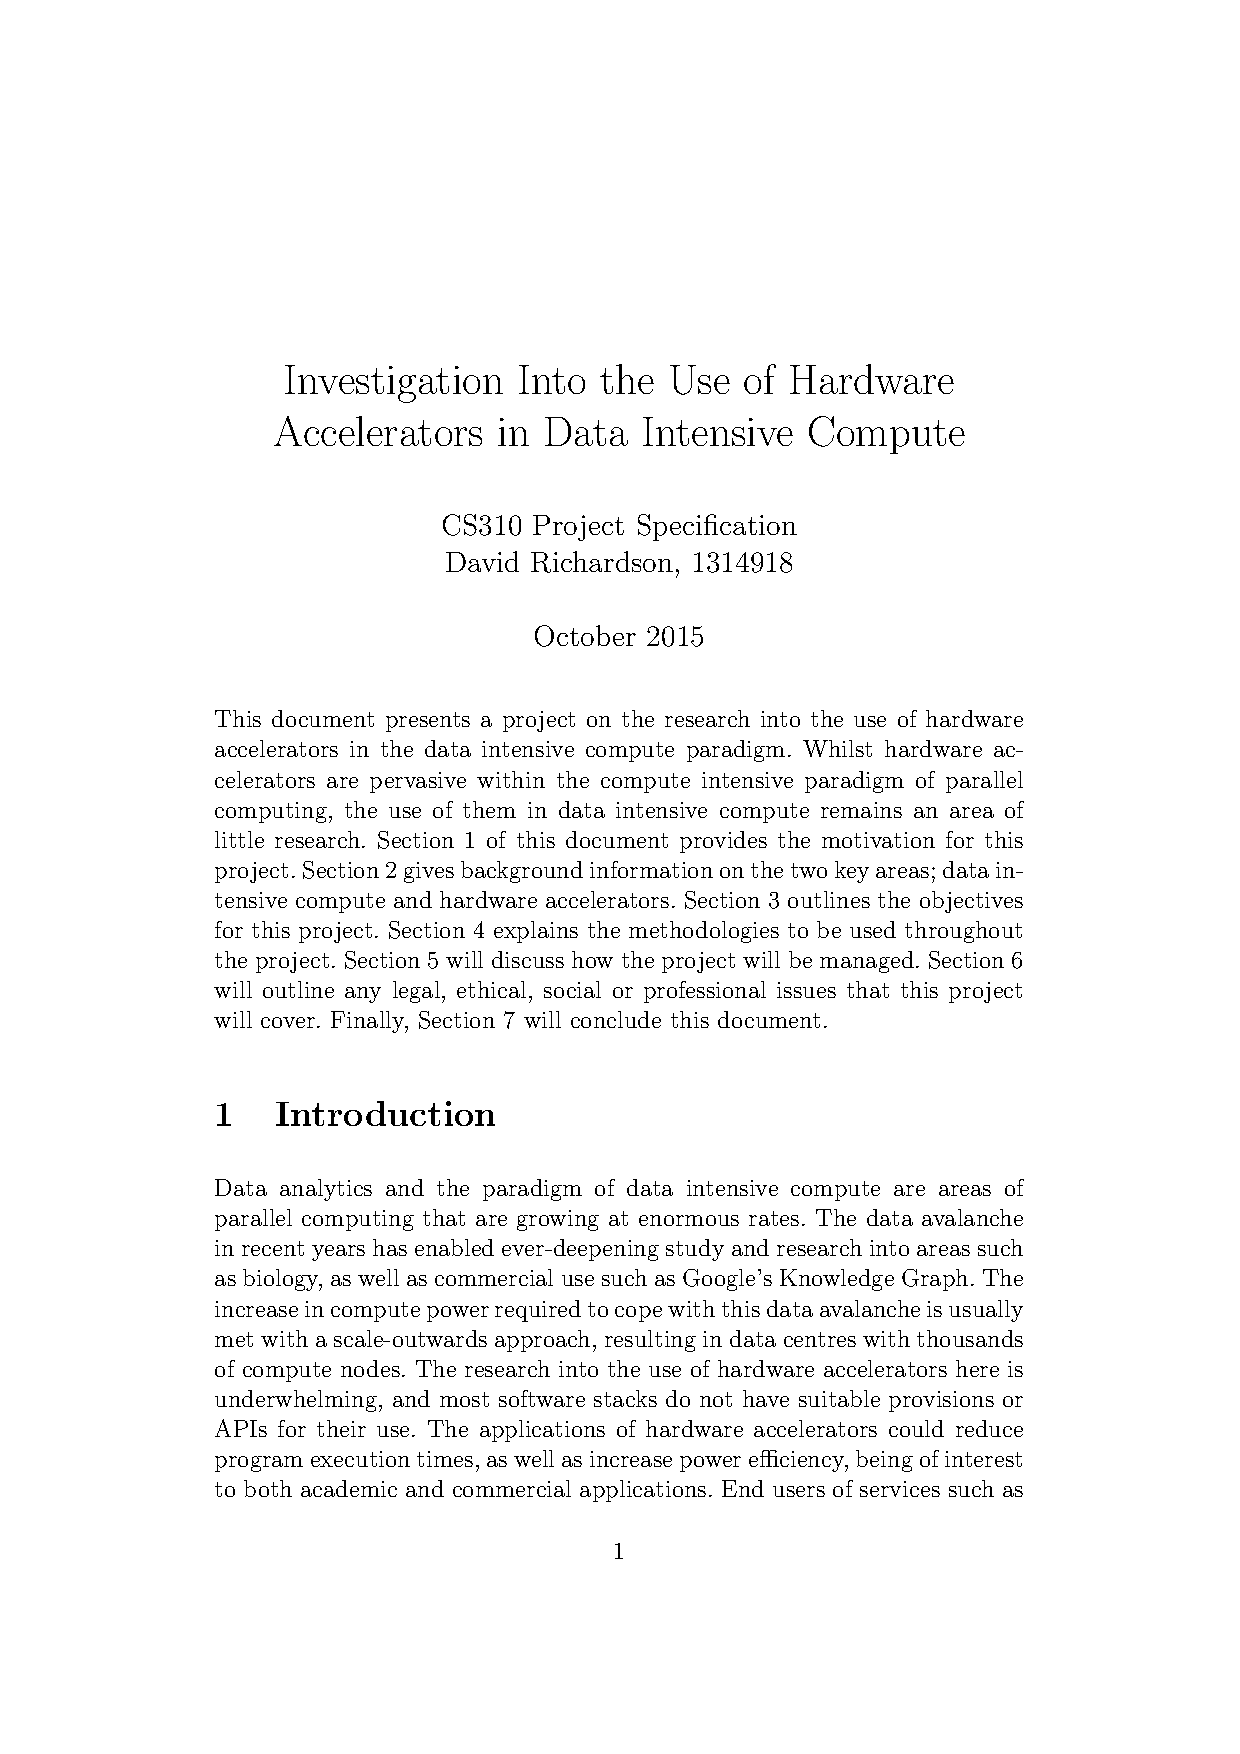
\includepdf[pages={1-12}, templatesize={16cm}{25.5cm}, frame=true]{specification.pdf}
	\end{appendices}

\end{document}